\documentclass{article}
\usepackage[top=3cm, bottom=3cm, left = 2cm, right = 2cm]{geometry} 
\geometry{a4paper} 
\usepackage[T1]{polski}
\usepackage[utf8]{inputenc}
\usepackage{titling}
\usepackage{caption}
\usepackage{algorithm}
\usepackage{algpseudocode}
\usepackage[parfill]{parskip}
\usepackage{multirow}
\usepackage{graphicx}
\usepackage{tikz}
\usepackage{pgfplots}
\usepgfplotslibrary{fillbetween}
\pgfplotsset{compat=1.18} 
\usepackage{amsmath}

\renewcommand\maketitlehooka{\null\mbox{}\vfill}
\renewcommand\maketitlehookd{\vfill\null}

\floatname{algorithm}{Algorytm}
\algrenewcommand\algorithmicrequire{\textbf{Dane:}}
\algrenewcommand\algorithmicensure{\textbf{Wyniki:}}

\title{Obliczenia Naukowe}
\author{Karol Janic}
\date{16 listopada 2023}

\begin{document}

\begin{titlingpage}
    \maketitle
\end{titlingpage}

\tableofcontents

\newpage

\section{Zadanie 1}
\subsection{Cel}
Celem zadania jest implementacja metody rozwiązującej równanie $f(x) = 0$ metodą bisekcji.

\subsection{Rozwiązanie}
\subsubsection{Opis metody}
Metoda służy znajdywaniu miejsca zerowego ciągłej funkcji $f$ na pewnym przedziale $[a, b]$. Wykorzystuje ona twierdzenie Darboux, 
które mówi że jeśli funkcja na końcach przedziału przyjmuje wartości o różnych znakach to w tym przedziale dla pewnego argumentu $r$ 
przyjmuje również wartość $0$. Metoda ta jest metodą iteracyjną i każdej kolejnej iteracji zmniejsza przedział poszukiwań o połowę. 
Robi to obliczając środek poprzedniego przedziału oraz wartość funkcji w tym punkcie. Następnie na podstawie znaku tej wartości 
wybiera prawy lub lewy podprzedział. Metoda kończy działanie, gdy wartość funkcji w środku przedziału jest wystarczająco bliska zeru($\epsilon$)
lub rozpatrywany przedział jest wystarczająco mały($\delta$).

\subsubsection{Uwagi implementacyjne}
\begin{itemize}
    \item sprawdzanie tego czy wartości funkcji na końcach przedziału mają różne znaki należy wykonać porównując znaki obu liczb 
    zamiast sprawdzania znaku ich iloczyny, ponieważ mnożenie bardzo małych liczb o różnych znakach może dać wynik zawierający się
    w przedziale zera maszynowego a mnożenie liczb bardzo dużych może doprowadzić do nadmiaru lub niedomiaru.
    \item wyznaczenie środka przedziału należy wykonać dodając połowę długości przedziału do jego lewego końca zamiast połowienia sumy końców oby przedziałów, 
    ponieważ błędy arytmetyki mogłyby spowodować, że środek przedziału zawierałby się poza przedziałem
\end{itemize}

\subsubsection{Wizualizacja metody}
\begin{tikzpicture}[scale=1]
    \draw[->] (-3.5,0) -- (1.5,0) node[right] {$x$};
    \draw[->] (0.5,-2) -- (0.5,4) node[above] {$f(x)$};

    \fill[blue, opacity=0.3] (-2,-1) rectangle (0,3);
    \fill[blue, opacity=0.3] (-1,-1) rectangle (0,1);
    \fill[blue, opacity=0.3] (-1,-0.375) rectangle (-0.5,1);
    
    \draw[domain=-3:1,smooth,variable=\x,black, line width=1pt] plot ({\x},{\x*\x*\x + 3*\x*\x - 1});
    
    \draw[dashed] (-2,3) -- (-2,0) node[below] {$a_1$};
    \draw[dashed] (0,-1) -- (0,0) node[above] {$b_1$};
    \draw[dashed] (-1,1) -- (-1,0) node[below] {$c_1$};
    \draw[dashed] (-0.5,-0.375) -- (-0.5,0) node[above] {$c_2$};
    \draw[dashed] (-0.75, 0.2565) -- (-0.75, 0) node[below] {$c_3$};

    \node[above right] at (1.5,3)   {warunek początkowy dla przedziału $[a_1, b_1]$ jest spełniony,};
    \node[above right] at (1.8,2.7) {ponieważ $f(a_1) \cdot f(b_1) < 0$};
    \node[above right] at (1.5,2.2) {iteracja 1: \quad $c_1 := \frac{a_1 + b_1}{2}$, \quad $f(a_1) \cdot f(c_1) > 0$ zatem $a_2 := c_1$ i $b_2 := b_1$};
    \node[above right] at (1.5,1.7) {iteracja 2: \quad $c_2 := \frac{a_2 + b_2}{2}$, \quad $f(a_2) \cdot f(c_2) < 0$ zatem $a_3 := a_2$ i $b_3 := c_2$};
    \node[above right] at (1.5,1.2) {iteracja 3: \quad $c_3 := \frac{a_3 + b_3}{2}$, \quad $f(a_3) \cdot f(c_3) < 0$ zatem $a_4 := a_3$ i $b_4 := c_3$};
    \node[above right] at (4.5,0.7) {$\vdots$};
\end{tikzpicture}

\newpage

\subsubsection{Pseudokod}
\begin{algorithm}[h!]
    \caption{Metoda bisekcji}
    \begin{algorithmic}[1]
        \Require $f$, \Comment{funkcja} \newline
        $a$, $b$, \Comment{przedział} \newline
        $\delta$, $\epsilon$    \Comment{dokładność obliczeń}
        \Ensure $c$, \Comment{przybliżenie pierwiastka równania $f(x) = 0$} \newline
         $f(c)$, \Comment{wartość funkcji $f$ w punkcie $c$ \newline}
         $it$, \Comment{liczba wykonanych iteracji} \newline
         $err$ \Comment{kod błędu}
        \Function{mbisekcji}{$f, a, b, \epsilon, \delta$}
            \State $fa \gets f(a)$
            \State $fb \gets f(b)$

            \If{$sign(fa) = sign(fb)$}
                \State \Return $0, 0, 0, 1$ \Comment{funkcja nie zmienia znaku na zadanym przedziale}
            \EndIf

            \State $e \gets b-a$
            \State $it \gets 0$
            \While{true}
                \State $it \gets it+1$
                \State $e \gets e/2$
                \State $c \gets a+e$
                \State $fc \gets f(c)$
                \If{$abs(e) < \delta \; or \; abs(fc) < \epsilon$}
                    \State \textbf{return} $c, fc, it, 0$ \Comment{znaleziono pierwiastek z zadaną dokładnością}
                \EndIf
                \If{$sign(fa) = sign(fc)$}  \Comment{wybieramy podprzedział tak aby zachować różne znaki}
                    \State $a \gets c$
                    \State $fa \gets fc$
                \Else
                    \State $b \gets c$
                    \State $fb \gets fc$
                \EndIf
            \EndWhile
        \EndFunction
    \end{algorithmic}
\end{algorithm}

\section{Zadanie 2}
\subsection{Cel}
Celem zadania jest implementacja metody rozwiązującej równanie $f(x) = 0$ metodą stycznych.

\subsection{Rozwiązanie}
\subsubsection{Opis metody}
Metoda służy znajdywaniu miejsca zerowego ciągłej, podwójnie różniczkowalnej funkcji $f$ o pochodnej $pf$
takiej, że $pf(r) \ne 0$, gdzie $r$ jest jednokrotnym pierwiastkiem. Wykorzystuje ona rozwinięcie funkcji $f$ w szereg Taylora 
w jej miejscu zerowym $r$ w celu jej linealizacji:
\[ 0 = f(r) = f(x_n) + pf(x_n)(r - x_n) + O((r-x_n)^2) \approx f(x_n) + pf(x_n)(r - x_n), \] 
skąd otrzymujemy wzór na kolejne przybliżenia pierwiastka:
\[ x_{n+1} = x_n - \frac{f(x_n)}{pf(x_n)} \]
Łatwo zauważyć, że wartością $x_{n+1}$ jest punkt przecięcia stycznej do wykresu funkcji $f$ w punkcie $(x_n, f(x_n))$ z osią $OX$.
Metoda ma charakter iteracyjny. Kolejne iteracje wyznacząją kolejne przybliżenia pierwiastka według podane wyżej wzoru.
Metoda kończy działanie, gdy różnica pomiędzy kolejnymi przybliżeniami jest dostatecznie mała($\delta$) lub wartość funkcji w przybliżeniu jest dostatecznie bliska zeru($\epsilon$). 
Ważnym założeniem jest także to, aby przybliżenie początkowe $x_0$ było dostatecznie bliskie dokładnemu zeru funkcji. W przeciwnym wypadku możemu nie zbliżać się do wartości dokładnej.
Aby metoda nie działała w nieskończoność warto zabezpieczyć ją poprzez wykonanie jedynie maksymalnie dopuszczalnej liczby iteracji($maxit$).

\subsubsection{Uwagi implementacyjne}
\begin{itemize}
    \item wyznaczenie kolejnego przybliżenia wymaga dzielenia przez wartość pochodnej funkcji $pf$; gdy jest ona bliska $0$ to wynik dzielenia może być odległy od rzeczywistej wartości 
    co może skutkować opuszczeniem bliskiego otoczenie wyznaczanego miejsca zerowego; należy się przed tym zabezpieczyć
\end{itemize}

\subsubsection{Pseudokod}
\begin{algorithm}[h!]
    \caption{Metoda stycznych}
    \begin{algorithmic}[1]
        \Require $f$, $pf$, \Comment{funkcja i jej pochodna} \newline
        $x_0$, \Comment{przybliżenie początkowe} \newline
        $maxit$, \Comment{maksymalna liczba iteracji} \newline
        $\delta$, $\epsilon$    \Comment{dokładność obliczeń}
        \Ensure $c$, \Comment{przybliżenie pierwiastka równania $f(x) = 0$} \newline
         $f(c)$, \Comment{wartość funkcji $f$ w punkcie $c$ \newline}
         $it$, \Comment{liczba wykonanych iteracji} \newline
         $err$ \Comment{kod błędu}
        \Function{mstycznych}{$f, pf, x_0, \epsilon, \delta$}
            \State $fx \gets f(x_0)$

            \If{$abs(fx) < \epsilon$}
                \State \Return $x_0, fx, 0, 0$ \Comment{dane przybliżenie początkowe jest wystarczająco dobre}
            \EndIf

            \State $x \gets x_0$
            \For{$it \gets 1$ \textbf{to} $\text{maxit}$}
                \State $dfx \gets pf(x)$
                \If{$abs(dfx) < 10.0 \cdot \text{eps}(\text{Float64})$}
                    \State \textbf{return} $x, fx, it, 2$   \Comment{wartość pochodnej jest bliska zeru}
                \EndIf
                \State $newx \gets x - fx / dfx$
                \State $fx \gets f(newx)$
                \If{$abs(newx - x)< \delta \; or \; abs(fx) < \epsilon$}
                    \State \textbf{return} $newx, fx, it, 0$
                \EndIf
                \State $x \gets newx$
            \EndFor
            \State \Return $x, fx, maxit, 1$ \Comment{nie udało znaleźć się wystarczająco dobre rozwiązania w $maxit$}
        \EndFunction
    \end{algorithmic}
\end{algorithm}

\newpage

\subsubsection{Wizualizacja metody}
\begin{tikzpicture}[scale=1]
    \draw[->] (-1.5,0) -- (4,0) node[right] {$x$};
    \draw[->] (-0.5,-1) -- (-0.5,6.5) node[above] {$f(x)$};

    \coordinate (A) at (3,0);
    \coordinate (B) at (1.846, 0);
    \coordinate (C) at (1.043, 0);
    \coordinate (D) at (0.721, 0);
    \coordinate (E) at (0.68, 0);
    \coordinate (F) at (3,4);
    \coordinate (G) at (1.84, 1.234);
    \coordinate (H) at (1.04, 0.283);
    \coordinate (B2) at (1.702, -0.5);
    \coordinate (C2) at (0.72, -0.5);
    \coordinate (D2) at (0.159, -0.5);
    \coordinate (F2) at (3.75,6.589);
    \coordinate (G2) at (3.75, 4.193);
    \coordinate (H2) at (3.75, 2.694);

    \fill[color=blue, opacity=0.3] (A) -- (F) -- (B) -- cycle;
    \fill[color=blue, opacity=0.6] (B) -- (G) -- (C) -- cycle;
    \fill[color=blue, opacity=0.9] (C) -- (H) -- (D) -- cycle;

    \draw[domain=-1:3.5,smooth,variable=\x,black, line width=1pt] plot ({\x},{0.624 * (2^\x) - 1}); 

    \draw[color=blue, opacity=0.3, line width=1.5pt] (F2) -- (B2);
    \draw[color=blue, opacity=0.6, line width=1.5pt] (G2) -- (C2);
    \draw[color=blue, opacity=0.9, line width=1.5pt] (H2) -- (D2);

    \draw[dashed, line width=0.6pt, black] (F) -- (A) node[below] {$x_0$};
    \node[above left] at (F) {$f(x_0)$};
    \fill (A) circle (2pt);
    \fill (F) circle (2pt);
    \draw[dashed, line width=0.6pt, black] (G) -- (B) node[below] {$x_1$};
    \node[above left] at (G) {$f(x_1)$};
    \fill (B) circle (2pt);
    \fill (G) circle (2pt);
    \draw[dashed, line width=0.6pt, black] (H) -- (C) node[below] {$x_2$};
    \node[above left] at (H) {$f(x_2)$};
    \fill (C) circle (2pt);
    \fill (H) circle (2pt);
    \draw[dashed, line width=0.6pt, black] (E) -- (E) node[below] {$x_3$};
    \fill (E) circle (2pt);

    \node[above right] at (4.5,6)         {iteracja 1: wyznaczamy styczną do wykresu funkcji w punkcie $(x_0,f(x_0))$,};
    \node[above right] at (6.0,5.6)       {przecięcie stycznej z osią $OX$ wyznacza kolejne przybliżenie $x_1$};
    \node[above right] at (4.5,4.9)       {iteracja 2: wyznaczamy styczną do wykresu funkcji w punkcie $(x_1,f(x_1))$,};
    \node[above right] at (6.0,4.5)       {przecięcie stycznej z osią $OX$ wyznacza kolejne przybliżenie $x_2$};
    \node[above right] at (4.5,3.8)       {iteracja 3: wyznaczamy styczną do wykresu funkcji w punkcie $(x_2,f(x_2))$,};
    \node[above right] at (6.0,3.4)       {przecięcie stycznej z osią $OX$ wyznacza kolejne przybliżenie $x_3$};
    \node[above right] at (8.5,2.7)       {$\vdots$};
\end{tikzpicture}

\section{Zadanie 3}
\subsection{Cel}
Celem zadania jest implementacja metody rozwiązującej równanie $f(x) = 0$ metodą siecznych.

\subsection{Rozwiązanie}
\subsubsection{Opis metody}
Metoda służy znajdywaniu miejsca zerowego ciągłej, podwójnie różniczkowalnej funkcji $f$, takiej że $f'(r) \ne 0$,
gdzie $r$ jest jednokrotnym pierwiastkiem równania. Jest ona ulepszoną metodą stycznych poprzez wyeliminowanie 
potrzeby używania pochodnej funkcji poprzez aproksymację:
\[ f'(x_{n}) \approx \frac{f(x_{n}) - f(x_{n-1})}{x_{n}-x_{n-1}} \]
W wyniku podstawienia otrzymujemy wzór rekurencyjny na kolejne przybliżenia pierwiastka:
\[ x_{n+1} = x_n - \frac{f(x_{n}) - f(x_{n-1})}{x_{n}-x_{n-1}} \cdot f(x_n) \]
W zamian za nieużywanie wzóru pochodnej funkcji potrzebujemy na początku dwa przybliżenia pierwiastka $x_0$, $x_1$.
Metoda ma charakter iteracyjny. Kolejne iteracje wyznacząją kolejne przybliżenia pierwiastka według podane wyżej wzoru.
Metoda kończy działanie, gdy różnica pomiędzy kolejnymi przybliżeniami jest dostatecznie mała($\delta$) lub wartość funkcji w przybliżeniu jest dostatecznie bliska zeru($\epsilon$). 
Ważnym założeniem jest także to, aby przybliżenia początkowe $x_0$, $x_1$ były dostatecznie bliskie dokładnemu zeru funkcji. W przeciwnym wypadku możemu nie zbliżać się do wartości dokładnej.
Aby metoda nie działała w nieskończoność warto zabezpieczyć ją poprzez wykonanie jedynie maksymalnie dopuszczalnej liczby iteracji($maxit$).

\subsubsection{Uwagi implementacyjne}
\begin{itemize}
    \item aby zapewnić, że wartość bezwzględna funkcji nie będzie rosła, przy wyznaczeniu kolejnych przybliżej 
    należy tak zamieniać $x_k$ oraz $x_{k+1}$ aby $|f(x_k)| \leq |f(x_{k+1})|$
\end{itemize}

\newpage

\subsubsection{Wizualizacja metody}
\begin{tikzpicture}[scale=1]
    \draw[->] (-1.5,0) -- (4,0) node[right] {$x$};
    \draw[->] (-0.5,-1) -- (-0.5,6.5) node[above] {$f(x)$};

    \coordinate (A) at (3,0);
    \coordinate (B) at (1.846, 0);
    \coordinate (C) at (1.322, 0);
    \coordinate (D) at (0.89, 0);
    \coordinate (E) at (0.68, 0);
    \coordinate (F) at (3,4);
    \coordinate (G) at (1.84, 1.234);
    \coordinate (H) at (1.322, 0.561);
    \coordinate (I) at (0.89, 0.157);
    \coordinate (X1) at (1.11, -0.51);
    \coordinate (Y1) at (3.75, 5.788);
    \coordinate (X2) at (0.5, -0.51);
    \coordinate (Y2) at (3.75, 3.72);

    \fill[color=blue, opacity=0.3] (A) -- (F) -- (G) -- (B) -- cycle;
    \fill[color=blue, opacity=0.6] (G) -- (B) -- (C) -- (H) -- cycle;
    \fill[color=blue, opacity=0.9] (C) -- (H) -- (I) -- (D) -- cycle;

    \draw[domain=-1:3.5,smooth,variable=\x,black, line width=1pt] plot ({\x},{0.624 * (2^\x) - 1}); 

    \draw[color=blue, opacity=0.3, line width=1.5pt] (X1) -- (Y1);
    \draw[color=blue, opacity=0.6, line width=1.5pt] (X2) -- (Y2);

    \draw[dashed, line width=0.6pt, black] (F) -- (A) node[below] {$x_0$};
    \node[above left] at (F) {$f(x_0)$};
    \fill (A) circle (2pt);
    \fill (F) circle (2pt);

    \draw[dashed, line width=0.6pt, black] (G) -- (B) node[below] {$x_1$};
    \node[above left] at (G) {$f(x_1)$};
    \fill (B) circle (2pt);
    \fill (G) circle (2pt);

    \draw[dashed, line width=0.6pt, black] (H) -- (C) node[below] {$x_2$};
    \node[above left] at (H) {$f(x_2)$};
    \fill (H) circle (2pt);
    \fill (C) circle (2pt);

    \fill (D) circle (2pt);
    \draw[dashed, line width=0.6pt, black] (D) -- (D) node[below] {$x_3$};

    \node[above right] at (4.5,6)         {iteracja 1: wyznaczamy sieczną przez punkty $(x_0,f(x_0))$ i $(x_1,f(x_1))$,};
    \node[above right] at (6.0,5.6)       {przecięcie siecznej z osią $OX$ wyznacza kolejne przybliżenie $x_2$};
    \node[above right] at (4.5,4.9)       {iteracja 2: wyznaczamy sieczną przez punkty $(x_1,f(x_1))$ i $(x_2,f(x_2))$,};
    \node[above right] at (6.0,4.5)       {przecięcie siecznej z osią $OX$ wyznacza kolejne przybliżenie $x_3$};
    \node[above right] at (8.5,3.8)       {$\vdots$};
\end{tikzpicture}

\subsubsection{Pseudokod}
\begin{algorithm}[h!]
    \caption{Metoda siecznych}
    \begin{algorithmic}[1]
        \Require $f$, \Comment{funkcja} \newline
        $x_0$, $x_1$ \Comment{przybliżenia początkowe} \newline
        $maxit$, \Comment{maksymalna liczba iteracji} \newline
        $\delta$, $\epsilon$    \Comment{dokładność obliczeń}
        \Ensure $c$, \Comment{przybliżenie pierwiastka równania $f(x) = 0$} \newline
         $f(c)$, \Comment{wartość funkcji $f$ w punkcie $c$ \newline}
         $it$, \Comment{liczba wykonanych iteracji} \newline
         $err$ \Comment{kod błędu}
        \Function{msiecznych}{$f, x_0, x_1, \epsilon, \delta$}
            \State $fx0 \gets f(x_0)$
            \State $fx1 \gets f(x_1)$

            \For{$it \gets 1$ \textbf{to} $\text{maxit}$}
                \If{$abs(fxo) > abs(fx1)$}
                    \State \textbf{swap(}$x_0, x_1$\textbf{)} 
                    \State \textbf{swap(}$fx0, fx1$\textbf{)} 
                \EndIf

                \State $s \gets (x_1 - x_0) / (fx1 - fx0)$
                \State $x_1 \gets x_0$
                \State $fx1 \gets fx0$
                \State $x_0 \gets x_0 - fx0 \cdot s$
                \State $fx0 \gets f(x_0)$
                
                \If{$abs(x_1 - x_0)< \delta \; or \; abs(fx0) < \epsilon$}
                    \State \textbf{return} $x_0, fx0, it, 0$
                \EndIf
            \EndFor
            \State \Return $x_0, fx0, maxit, 1$ \Comment{nie udało znaleźć się wystarczająco dobre rozwiązania w $maxit$}
        \EndFunction
    \end{algorithmic}
\end{algorithm}

\section{Zadanie 4}
\subsection{Cel}
Celem zadania jest przetestowanie zaimplementowanych metod na przykładzie funkcji $f_0(x) = \sin{x} - (\frac{x}{2})^2$
\subsection{Rozwiązanie}
\begin{figure}[h!]
    \centering
    \begin{tikzpicture}[scale=1]
        \draw[->] (-5,0) -- (5,0) node[right] {$x$};
        \draw[->] (0,-4.5) -- (0,2.5) node[above] {$y$};

        \foreach \x in {-4, -3, -2, -1, 0, 1, 2, 3, 4}
            \draw (\x,0.1) -- (\x,-0.1) node[below] {\x};
        
        \foreach \y in {-4, -3, -2, -1, 1, 2}
            \draw (0.1,\y) -- (-0.1,\y) node[left] {\y};
            
        \draw[blue, opacity=0.9, thick, domain=-4:4, samples=100] plot (\x, {sin(\x r) - (\x/2)^2});
        \draw[purple, opacity=0.9, thick, domain=-4:4, samples=100] plot (\x, {cos(\x r) - (\x/2)});
        
        \node[align=center, text width=2cm] at (2, 0.7) {$f_0(x)$};
        \node[align=center, text width=2cm] at (-1, 1.5) {$f'_0(x)$};
    \end{tikzpicture}
    \caption{Wizualizacja $f_0(x) = \sin{x} - (\frac{x}{2})^2$ oraz $f'_0(x) = \cos{x} - \frac{x}{2}$ }
\end{figure}

Użyto zaimplementowanych wcześniej metod z podanymi poniżej argumentami:
\begin{itemize}
    \item \textbf{mbisekcji:} $a := 1.5$, $b := 2.0$, $delta := 0.5 \cdot 10^{-5}$, $epsilon := 0.5 \cdot 10^{-5}$
    \item \textbf{mstycznych:} $x0 := 1.5$, $delta := 0.5 \cdot 10^{-5}$, $epsilon := 0.5 \cdot 10^{-5}$, $maxit := 1024$
    \item \textbf{msiecznych:} $x0 := 1.0$, $x1 := 2.0$, $delta := 0.5 \cdot 10^{-5}$, $epsilon := 0.5 \cdot 10^{-5}$, $maxit := 1024$
\end{itemize}

\subsection{Wyniki}
\begin{table}[h!]
    \centering
    \begin{tabular}{|c|c|c|c|c|}
    \hline
    \textbf{Metoda} & \textbf{Wyznaczony pierwiastek} & \textbf{Wartość funkcji w pierwiastku} & \textbf{Liczba iteracji} & \textbf{Kod błędu} \\
    \hline
    mbisekcji & 1.9337539672851562 & -2.7027680138402843e-7 & 16 & 0 \\
    \hline
    mstycznych & 1.933753779789742 & -2.2423316314856834e-8 & 4 & 0 \\
    \hline
    msiecznych & 1.933753644474301 & 1.564525129449379e-7 & 4 & 0 \\
    \hline
    \end{tabular}
    \caption{Wyniki eksperymentów dla $f_0(x) = \sin{x} - (\frac{x}{2})^2$}
\end{table}

\subsection{Wnioski}
\begin{itemize}
    \item używając metody bisekcji, stycznych oraz siecznych z podobnymi parametrami początkowymi i taką samą zadaną dokładnością 
    otrzymano bliskie sobie wartości pierwiastka rozwiązywanego równania
    \item wartości najbliższe wartościom dokładnym otrzymano przy pomocy metody stycznych
    \item metoda bisekcji potrzebowała największej liczby iteracji do otrzymania wyniki; jest to zgodne z oczekiwaniami, 
    ponieważ jej współczynnik zbieżności wynosi $2$, metody stycznych $1$ a metody siecznych $\approx 1.6$
    \item znając pochodną funkcji, bliskie przybliżenie szukanego pierwiastka oraz wiedząc, że pochodna jest "dobra" warto użyć metody stycznych
\end{itemize}

\newpage

\section{Zadanie 5}
\subsection{Cel}
Celem zadania jest znalezienie wartości $x$ dla których wykresy funkcji $y = 3x$ oraz $y = e^x$ przecinają się.

\subsection{Rozwiązanie}
\begin{figure}[h!]
    \centering
    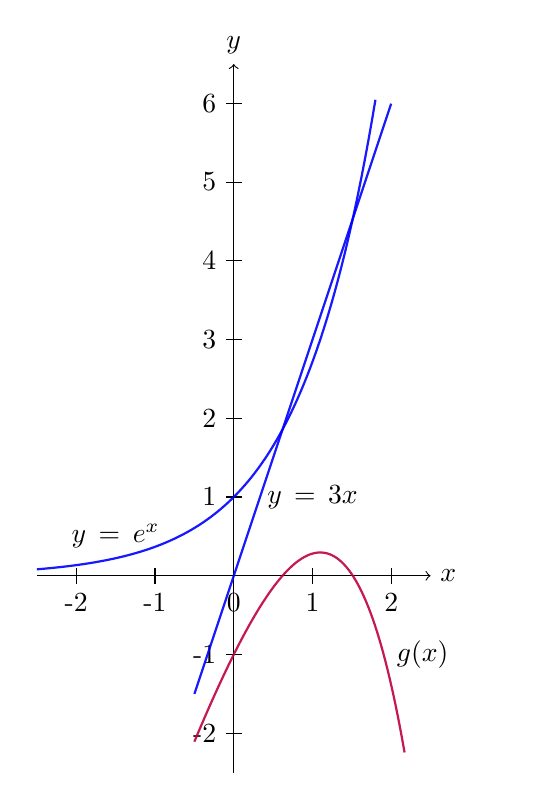
\begin{tikzpicture}[scale=1]
        \draw[->] (-2.5,0) -- (2.5,0) node[right] {$x$};
        \draw[->] (0,-2.5) -- (0,6.5) node[above] {$y$};

        \foreach \x in {-2, -1, 0, 1, 2}
            \draw (\x,0.1) -- (\x,-0.1) node[below] {\x};
        
        \foreach \y in {-2, -1, 1, 2, 3, 4, 5, 6}
            \draw (0.1,\y) -- (-0.1,\y) node[left] {\y};
            
        \draw[blue, opacity=0.9, thick, domain=-0.5:2, samples=100] plot (\x, {3*\x});
        \draw[blue, opacity=0.9, thick, domain=-2.5:1.8, samples=100] plot (\x, {exp(\x)});
        \draw[purple, opacity=0.9, thick, domain=-0.5:2.17, samples=100] plot (\x, {3*\x - exp(\x)});
        
        \node[align=center, text width=2cm] at (1, 1) {$y = 3x$};
        \node[align=center, text width=2cm] at (-1.5, 0.5) {$y = e^x$};
        \node[align=center, text width=2cm] at (2.4, -1) {$g(x)$};
    \end{tikzpicture}
    \caption{Wizualizacja $y=3x$, $y=e^x$, $g(x) = 3x - e^x$}
\end{figure}

Na podstawie wizualizacji funkcji $g(x) = 3x - e^x$ określono przedziały w których znajdują się miejsca zerowe tej funkcji, 
które są argumentami dla których wykresy funkcji o wzorach $3x$ oraz $e^x$ przecinają się.  \newline
Dla przedziałów $[0.0, 1.0]$, $[1.0, 2.0]$ i dokładności $delta = epsilon = 10^{-4}$ użyto metody bisekcji.

\subsection{Wyniki}
\begin{table}[h!]
    \centering
    \begin{tabular}{|c|c|c|c|c|c|c|}
    \hline
    \multirow{2}{*}{\textbf{Przedział}} & \textbf{Wyznaczony} & \multirow{2}{*}{$\textbf{g(r)}$} & \textbf{Liczba} & \textbf{Kod} & \multirow{2}{*}{$\textbf{3r}$} & \multirow{2}{*}{$\textbf{e}^\textbf{r}$} \\
    & \textbf{pierwiastek} $\textbf{r}$ & & \textbf{iteracji} & \textbf{błędu} & & \\
    \hline
    $[0.0, 1.0]$ & 0.619140625 & -9.066320343276146e-5 & 9 & 0 & 1.8573312117965672 & 1.857421875 \\
    \hline
    $[1.0, 2.0]$ & 1.51171875 & -0.000638447089475136 & 8 & 0 & 4.534517802910525 & 4.53515625 \\
    \hline
    $[0.0, 2.0]$ & - & - & - & 1 & - & - \\
    \hline
    \end{tabular}
    \caption{Wyniki eksperymentów dla $f_0(x) = \sin{x} - (\frac{x}{2})^2$}
\end{table}

\subsection{Wnioski}
\begin{itemize}
    \item metoda bisekcji poprawnie znajduje miejsce przecięcia dwóch funkcji po zapisaniu ich w odpowiedniej formie
    \item metoda wymaga uprzedniej analizy badanej funkcji, tj. znalezienia podprzedziałów, w których występuje zero funkcji 
    oraz których końce mają rożne znaki wartości funkcji - tego warunku nie spełnia przedział $[0.0, 2.0]$
\end{itemize}

\newpage

\section{Zadanie 6}
\subsection{Cel}
Celem zadania jest znalezienie miejsc zerowych funkcji  $f_1(x) = e^{1-x} - 1$ oraz $f_2(x) = x e^{-x}$

\subsection{Rozwiązanie}
\begin{figure}[h!]
    \centering
    \begin{tikzpicture}[scale=1]
        \draw[->] (-1.5,0) -- (7.5,0) node[right] {$x$};
        \draw[->] (0,-3.5) -- (0,4.5) node[above] {$y$};

        \foreach \x in {-1, 0, 1, 2, 3, 4, 5, 6, 7}
            \draw (\x,0.1) -- (\x,-0.1) node[below] {\x};
        
        \foreach \y in {-3, -2, -1, 1, 2, 3, 4}
            \draw (0.1,\y) -- (-0.1,\y) node[left] {\y};
            
        \draw[blue, opacity=0.9, thick, domain=-0.5:7, samples=100] plot (\x, {exp(1-\x) - 1});
        \draw[purple, opacity=0.9, thick, domain=-0.3:7, samples=100] plot (\x, {-exp(-\x + 1)});
        
        \node[align=center, text width=2cm] at (5, -1.5) {$f_1(x)$};
        \node[align=center, text width=2cm] at (5, 0.5) {$f'_1(x)$};
    \end{tikzpicture}
    \caption{Wizualizacja $f_1(x) = e^{1-x} - 1$ oraz $f'_1(x) = -e^{1-x}$}
\end{figure}

\vspace{1cm}

\begin{figure}[h!]
    \centering
    \begin{tikzpicture}[scale=1]
        \draw[->] (-1.5,0) -- (7.5,0) node[right] {$x$};
        \draw[->] (0,-2.5) -- (0,3.5) node[above] {$y$};

        \foreach \x in {-1, 0, 1, 2, 3, 4, 5, 6, 7}
            \draw (\x,0.1) -- (\x,-0.1) node[below] {\x};
        
        \foreach \y in {-2, -1, 1, 2, 3}
            \draw (0.1,\y) -- (-0.1,\y) node[left] {\y};
            
        \draw[blue, opacity=0.9, thick, domain=-0.5:7, samples=100] plot (\x, {\x * exp(-\x)});
        \draw[purple, opacity=0.9, thick, domain=-0.3:7, samples=100] plot (\x, {exp(-\x) - \x * exp(-\x)});
        
        \node[align=center, text width=2cm] at (2, 0.7) {$f_2(x)$};
        \node[align=center, text width=2cm] at (2, -0.7) {$f'_2(x)$};
    \end{tikzpicture}
    \caption{Wizualizacja $f_2(x) = xe^{-x}$ oraz $f'_2(x) = e^{-x} - xe^{-x}$}
\end{figure}

\vspace{1cm}

Przetestowano zaimplementowane funkcje dla różnych dany początkowych oraz $delta = epsilon = 10^{-5}$.

\newpage

\subsection{Wyniki}
\subsubsection{Metoda bisekcji dla $f_1(x)$}
\begin{table}[h!]
    \centering
    \begin{tabular}{|c|c|c|c|c|c|}
    \hline
    \textbf{a} & \textbf{b} & \textbf{Wyznaczone zero} & \textbf{Wartość w  zerze} & \textbf{Liczba iteracji} & \textbf{Kod błędu} \\
    \hline
    0.0 & 2.0 & 1.0 & 0.0 & 1 & 0 \\
    \hline
    -1.0 & 5.0 & 1.00006103515625 & -6.1033293642709374e-5 & 15 & 0 \\
    \hline
    1.0 & 512.0 & 1.0000609159469604 & -6.0914091621788735e-5 & 23 & 0 \\
    \hline
    256.5 & -256.5 & 0.9999961853027344, & 3.814704541582614e-6 & 18 & 0 \\
    \hline
    $-5.0 \cdot 10^{6}$ & $5.0 \cdot 10^{6}$ & 1.00000761449337 & -7.614464379912533e-6 & 33 & 0 \\
    \hline    
\end{tabular}
    %\caption{Wyniki eksperymentów metody dla bisekcji oraz $f_1(x)$}
\end{table}

\subsubsection{Metoda bisekcji dla $f_2(x)$}
\begin{table}[h!]
    \centering
    \begin{tabular}{|c|c|c|c|c|c|}
    \hline
    \textbf{a} & \textbf{b} & \textbf{Wyznaczone zero} & \textbf{Wartość w  zerze} & \textbf{Liczba iteracji} & \textbf{Kod błędu} \\
    \hline
    -5.0 & 5.0 & 0.0 & 0.0 & 1 & 0 \\
    \hline
    -3.0 & 7.0 & 3.0517578125e-5 & 3.0516646816636094e-5 & 16 & 0 \\
    \hline
    0.0 & 10.0 & 7.62939453125e-5 & 7.628812476844761e-5 & 17 & 0 \\
    \hline 
    -3.0 & 0.0 & -9.1552734375e-5 & -9.156111666187633e-5 & 15 & 0 \\
    \hline 
    -2.0 & 1024.0 & 511.0 & 6.0805189678747255e-220 & 1 & 0 \\
    \hline
    \end{tabular}
    %\caption{Wyniki eksperymentów dla metody bisekcji oraz $f_2(x)$}
\end{table}

\subsubsection{Metoda stycznych dla $f_1(x)$}
\begin{table}[h!]
    \centering
    \begin{tabular}{|c|c|c|c|c|}
    \hline
    \textbf{x0} & \textbf{Wyznaczone zero} & \textbf{Wartość w  zerze} & \textbf{Liczba iteracji} & \textbf{Kod błędu} \\
    \hline
    1.0 & 1.0 & 0.0 & 0 & 0 \\
    \hline
    0.0 & 0.9999984358892101 & 1.5641120130194253e-6 & 4 & 0 \\
    \hline
    -2.0 & 0.9999877637594053 & 1.223631545776982e-5 & 6 & 0 \\
    \hline
    -5.0 & 0.999984567543171 & 1.5432575910079294e-5 & 9 & 0 \\
    \hline
    -7.0 & 0.9999844095452799 & 1.5590576251778288e-5 & 11 & 0 \\
    \hline
    -10.0 & 0.9999843859457858 & 1.561417611428695e-5 & 14 & 0 \\
    \hline
    -512.0 & -256.0 & 4.10848635681094e111 & 256 & 1 \\
    \hline
    2.0 & 0.9999999810061002 & 1.8993900008368314e-8 & 5 & 0 \\
    \hline
    5.0 & 0.9999996427095682 & 3.572904956339329e-7 & 54 & 0 \\
    \hline
    7.0 & -140.4287934927351 & 2.640855242262125e61 & 256 & 1 \\
    \hline
    10.0 & NaN & NaN & 256 & 1 \\
    \hline
    512.0 & 512.0 & -1.0 & 1 & 2 \\
    \hline
    \end{tabular}
    %\caption{Wyniki eksperymentów dla metody stycznych oraz $f_1(x)$}
\end{table}

\subsubsection{Metoda stycznych dla $f_2(x)$}
\begin{table}[h!]
    \centering
    \begin{tabular}{|c|c|c|c|c|}
    \hline
    \textbf{x0} & \textbf{Wyznaczone zero} & \textbf{Wartość w  zerze} & \textbf{Liczba iteracji} & \textbf{Kod błędu} \\
    \hline
    0.0 & 0.0 & 0.0 & 0 & 0 \\
    \hline
    1.0 & 1.0 & 0.36787944117144233 & 1 & 2 \\
    \hline
    2.0 & 12.228417566135983 & 5.979102365781934e-5 & 8 & 0 \\
    \hline
    4.0 & 12.228417566135983 & 5.979102365781934e-5 & 7 & 0 \\
    \hline
    16.0 & 16.0 & 1.8005627955081459e-6 & 0 & 0 \\
    \hline
    256.0 & 256.0 & 1.6937628305176282e-109 & 0 & 0 \\
    \hline
    -1.0 & -3.0642493416461764e-7 & -3.0642502806087233e-7 & 5 & 0 \\
    \hline
    -2.0 & -3.775651605669814e-5 & -3.775794163811521e-5 & 6 & 0 \\
    \hline
    -4.0 & -1.5586599258811135e-6 & -1.5586623553037713e-6 & 9 & 0 \\
    \hline
    -16.0 & -2.0358324570344394e-5 & -2.0358739035942602e-5 & 22 & 0 \\
    \hline
    -256.0 & -4.042760404177798 & -230.3703269366329 & 256 & 1 \\
    \hline
    \end{tabular}
    %\caption{Wyniki eksperymentów dla metody stycznych oraz $f_2(x)$}
\end{table}

\newpage

\subsubsection{Metoda siecznych dla $f_1(x)$}
\begin{table}[h!]
    \centering
    \begin{tabular}{|c|c|c|c|c|c|}
    \hline
    \textbf{x0} & \textbf{x1} & \textbf{Wyznaczone zero} & \textbf{Wartość w  zerze} & \textbf{Liczba iteracji} & \textbf{Kod błędu} \\
    \hline
    0.0 & 1.0 & 1.0 & 0.0 & 1 & 0 \\
    \hline
    0.0 & 0.5 & 0.9999098501025039 & 9.015396112022067e-5 & 4 & 0 \\
    \hline
    -10.0 & -5.0 & 0.9999985625881762 & 1.43741285696386e-6 & 14 & 0 \\
    \hline
    -32.0 & 0.0 & 2.561689409277081e-13 & 1.7182818284583492 & 1 & 0 \\
    \hline
    1.5 & 3.0 & 0.9999997679008488 & 2.3209917809907665e-7 & 6 & 0 \\
    \hline
    2.0 & 4.0 & 0.9999881213444997 & 1.1878726051905986e-5 & 8 & 0 \\
    \hline
    2.0 & 16.0 & 1.9999999985244834 & -0.6321205582857454 & 2 & 0 \\
    \hline
    32.0 & 64.0 & 32.0 & -0.9999999999999656 & 2 & 0 \\
    \hline
    \end{tabular}
    %\caption{Wyniki eksperymentów dla metody siecznych oraz $f_1(x)$}
\end{table}

\subsubsection{Metoda siecznych dla $f_2(x)$}
\begin{table}[h!]
    \centering
    \begin{tabular}{|c|c|c|c|c|c|}
    \hline
    \textbf{x0} & \textbf{x1} & \textbf{Wyznaczone zero} & \textbf{Wartość w  zerze} & \textbf{Liczba iteracji} & \textbf{Kod błędu} \\
    \hline
    -1.0 & 0.0 & 0.0 & 0.0 & 1 & 0 \\
    \hline
    -2.0 & -1.0 & -6.982568902521766e-6 & -6.982617658960467e-6 & 7 & 0 \\
    \hline
    -8.0 & -4.0 & -4.594470908463521e-5 & -4.594682004942155e-5 & 13 & 0 \\
    \hline
    -16.0 & -1.0 & -0.999999713216569 & -2.718280269343002 & 1 & 0 \\
    \hline
    1.0 & 2.0 & 11.777830432946175 & 9.036880338187556e-5 & 10 & 0 \\
    \hline
    \end{tabular}
    %\caption{Wyniki eksperymentów dla metody siecznych oraz $f_2(x)$}
\end{table}

\subsection{Obserwacje}
\subsubsection{Metoda bisekcji}
\begin{itemize}
    \item gdy końce początkowego przedziału leżą symetrycznie względem miejsca zerowego funkcji to zbieżność jest natychmiastowa
    \item gdy długość początkowego przedziału rośnie to rośnie także liczba niezbędnych iteracji do znalezienia miejsca zerowe funkcji
    \item gdy przedział początkowy jest "bardziej symetryczny" względem pierwiastka funkcji to potrzebna jest mniejsza liczba iteracji do jego znalezienia
    \item gdy funkcja nie przyjmuje wartości bliskich $0$(bliskość określona poprzez podany do funkcji epsilon) to wynik metody dla dowolnie dużego przedziału jest poprawny
\end{itemize}

\subsubsection{Metoda stycznych}
\begin{itemize}
    \item gdy początkowe przybliżenie jest wystarczająco bliskie rzeczywistej wartości to metoda od razu zwraca wynik
    \item gdy początkowa wartość jest bliska rozwiązania rzeczywistego to metoda szybko zbiega
    \item gdy wartość funkcji jest bliska zera dla początkowego przybliżenia to metoda bardzo szybko zwraca niepoprawny wynik
    \item gdy wartość bezwzględna pochodnej osiąga duże wartości to styczna jest prawie pionowa i wówczas aby metoda zbiegła niezbędna jest bardzo duża liczba iteracji
    \item gdy wartość bezwzględna pochodnej osiąga wartości bliskie zeru, ale nie tak bliskie "aby metoda to wykryła" to styczna jest prawie pozioma a kolejne przybliżenia są bardzo dalekie od rzeczywistego pierwiastka funkcji, przez co metoda rozbiega
\end{itemize}

\newpage

\subsubsection{Metoda siecznych}
\begin{itemize}
    \item gdy jedno z przybliżeń początkowych jest wystarczająco bliskie rzeczywistej wartości to metoda od razu zwraca wynik
    \item gdy przybliżenia początkowe są bliskie rozwiązania rzeczywistego to metoda szybko zbiega
    gdy wartość funkcji jest bliska zera dla początkowego przybliżenia to metoda bardzo szybko zwraca niepoprawny wynik
    \item gdy kolejne początkowe przybliżenia oddalają się od siebie to rośnie liczba niezbędnych iteracji do uzyskania wyniku
    \item gdy wartość bezwzględna pochodnej osiąga duże wartości to kolejne sieczne są prawie pionowe i wówczas kolejne przybliżenia są sobie bardzo bliskie co skutkute przyjęciem błędnej wartości jako przybliżenie pierwiastka badanej funkcji
    \item gdy wartość bezwzględna pochodnej osiąga wartości bliskie zeru, to kolejne wartości funkcji są bliskie i wtedy następuje dzielenie przez rożnicę bliskich sobie liczb co może prowadzić do niedokładności i rozbiegania metody
\end{itemize}

\subsection{Wnioski}
\begin{itemize}
    \item metoda bisekcji jest zbieżna globalnie(z wyjątkami, gdy badana funkcja osiąga wartości bliskie zera) zaś metoda stycznych i siecznych jest zbieżna lokalnie
    \item metoda bisekcji(zbieżność kwadratowa) zbiega powoli zaś metoda stycznych(zbieżność liniowa) oraz metoda siecznych(współczynnik zbieżności $\approx 1.68$) zbiegają szybko
    \item przed użyciem powyższych metod należy zbadać funkcję, której pierwiastka szukamy aby odpowiednio dobrać pozostałe parametry metod
    \item w celu zapewnienia zbieżności i szybkości wyznaczania pierwiastka można używać powyższych metod hybrydowo - metodą bisekcji znaleźć pierwsze przybliżenie a następnie użyć metody stycznych lub siecznych do ich poprawienia
\end{itemize}

\end{document}
